\section{ZooProcess}

ZooProcess 是基于ImageJ 宏语言的一套程序。所以Zooprocess对用户来说是免费的,用户也可以用它来满足他们的需求。

Zooprocess 是由Marc Picheral 开发出来并且为我们所使用的,然而他并不是一名程序员。 Zooprocess 依旧在完善并且新的版本会在主页上发布出来。 我们认为\textbf{文件的格式和项目的结构}是不允许被修改的。但是上行的兼容性是会保持的。

\subsection{安装}
	\subsubsection{计算机规格}
		\begin{itemize}
			\item 不要使用双处理器的电脑,多核的电脑是支持的。
			\item 在Windows Xp 32操作系统上需要2G的内存来处理Zooscan 2400 dpi的图像。现在不再推荐这个已经被废弃的系统。
			\item 在Windows7 64位和Windows8操作系统需要最小8G的内存来处理 4800dpi的图像。
			\item 对于Zooscan来说分辨率最小是1280\*1024,这里推荐1680\*1280的分辨率,对查看图像来说是好的。对于ZOOSCAN工具来说最小的垂直分辨率是1024dpi,因此建议不要使用笔记本电脑。
			\item 一个带有滚轮按钮的鼠标对于很多的手动图像工具来说是必须的。			
		\end{itemize}
	\subsubsection{系统规格}
	
		Zooprocess 已经在这些系统上测试并且可以兼容他们:
		\begin{itemize}
			\item Windows XP pro 32bits, SP3。
			\item windows 7 pro 64 bits
			\item windows 8 pro 64 bits	
		\end{itemize}
	\subsubsection{操作系统区域设定}
		配置电脑使用点作为十进制的符号。如图~\ref{fig:systemconfig}
		\begin{figure}[!ht]
    		\centering
    		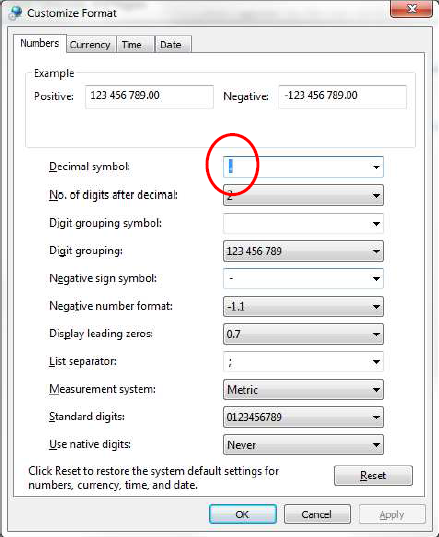
\includegraphics[width=5in]{ZooProcess_System_Config}
    		\caption{配置电脑}
    		\label{fig:systemconfig}
    		\end{figure}
	\subsubsection{使用过程中用的文件}
		提供的安装文件,可以到\url{http://www.obs-vlfr.fr/LOV/ZooPart/ZooScan/article.php3?id_article=218}下载安装文件,包含所有相关的文件及文档。
		
		在使用过程中会用到的软件:
		
		\begin{enumerate}
			\item 使用Zooscan时相关的软件
				\begin{itemize}
					\item Zooscan Driver
					\item Vuescan
					\item Java machine
					\item ImageJ and Zooprocess
					\item	First START of Zooporcess
					\item Tanagra 
					\item Pid Viewer
					\item PKId
					\item Xnview
				\end{itemize}
			\item 处理Zooscan 数据时相关的软件
				\begin{itemize}
					\item Vuescan
					\item Java machine
					\item ImageJ and Zooprocess
					\item First START of Zooprocess
					\item	Tangara
					\item Pid Viewer
					\item PKId
					\item XnView
				\end{itemize}
			\item 运行UVP相关的软件
				UVP(underwater vision profiler)系统,被设计用于对直径大于100um的课件颗粒和浮游生物的垂直分布进行量化。\href{http://www.doc88.com/p-1921921926742.html}{参考来源}
				\begin{itemize}
					\item Java machine
					\item ImageJ and Zooprocess
					\item RS232 piloting tools
					\item First START of Zooprocess
					\item	Tangara
					\item Pid Viewer
					\item PKId
					\item	XnView
				\end{itemize}
			\item 处理UVP数据时相关的软件
				\begin{itemize}
					\item Java machine
					\item ImageJ and Zooprocess 
					\item First START of Zooprocess
					\item Tangara
					\item	Pid Viewer
					\item PKId
					\item XnView
				\end{itemize}
			\item 其他软件
				\begin{itemize}
					\item Java machine
					\item ImageJ and Zooprocess
					\item First START of Zooprocess
					\item Tangara
					\item	Pid Viewer
					\item PKId
					\item XnView
				\end{itemize}
		\end{enumerate}
	\subsubsection{安装顺序}
		必须要按照说明的顺序去安装。
	
		下表~\ref{fig:systemfile}说明了不同系统安装的文件: 
		\begin{figure}[!ht]
    		\centering
    		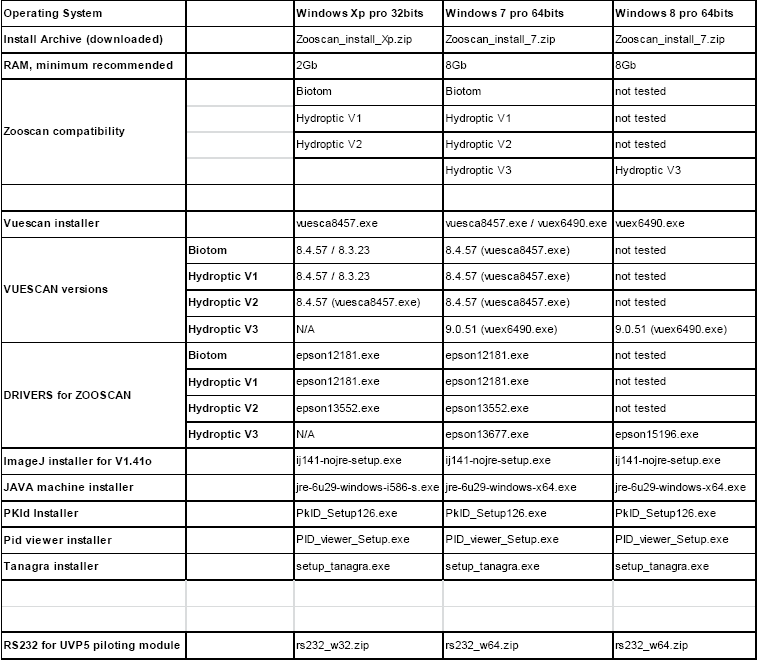
\includegraphics[width=7in]{ZooProcess_System_File}
    		\caption{不同系统安装的文件}
    		\label{fig:systemfile}
    		\end{figure}
		
		\begin{enumerate}
			\item 安装Zooscan驱动
				\begin{itemize}
					\item 根据上面列表,安装win7 64位对应的驱动(epsonxxxx.exe)
					\item 连接Zooscan
					\item 打开Zooscan并且检查是否安装成功
					\item 关闭Zooscan
				\end{itemize}
			\item 安装Vuescan
				\begin{itemize}
					\item 从下载的文件夹中打开安装文件
					\item 注意不要选“安装旧版本的驱动"
					\item 运行Vuescan并且输入许可信息(相关信息可以上网找序列号)
					\item	关闭
				\end{itemize}
			\item 安装JAVA
				用户必须通过提供的JAVA machines 运行ImageJ。永远不要升级JAVA。
				\begin{itemize}
					\item 在32位系统下只安装 jre-6u29-windows-i586-s.exe												\item 在64位系统下只安装 jre-6u29-windows-x64.exe
				\end{itemize}
				在安装的时候保持默认的选项。
			\item 安装 ImageJ
				
				只有1.41版本的ImageJ 会适用于 7.0以上版本的Zooprocess。
				
				64位系统下的安装过程:
				
				64位系统运行扫描和处理2400分辨率的大帧图像以及4800分辨率的窄帧图像需要在拥有8Gb的内存的前提下。对于更多的内存,并不会提高处理速度。
				\begin{itemize}
					\item 从提供的文件夹内安装ImageJ(ij141-nojre-setup.exe)。ImageJ 必须安装到用户有写权限的文件夹,例如桌面(Desktop/ImageJ)。
					\item 在弹出的窗口中定义已安装的java的路径(一般在C盘的program file 文件夹内)。
					\item 当计算机的防火墙提示JAVA时,允许其运行。
					\item 设置分配给ImageJ的内存空间为计算机内存的2/3。
					\item	关闭并重启ImageJ,查看设置是否生效。
				\end{itemize}
			\item 安装Zooprocess
				\begin{itemize}
					\item 如果ImageJ启动的话先关闭它。
					\item 解压缩Zooprocess\_version\_x.xx.zip压缩包内的所有内容到ImageJ下面的macros文件夹,替换掉原有的文件。
					\item 把free\_memory.class和free\_memory.java以及所有的扩展名为*.class和*.java的文件从ImageJ\\macros文件夹移动到ImageJ\\plugins文件夹内。
					\item Tangara
					\item	Pid Viewer
					\item PKId
					\item XnView
				\end{itemize}
			\item 安装Tanagra、PID viewer、Plankton Identifier和Xnview。
				从提供的文件夹内安装前三个软件,Xnview自己上网下载,任何版本都可以。
		\end{enumerate}
		
\subsection{启动和使用Zooprocess}

	\textbf{注意:}
	\begin{itemize}
		\item 在启动Zooprocess之前请关闭所有的应用程序。
		\item 在Zooprocess处理的过程中不要做其他任何事情。
		\item 第一次启动Zooprocess的时候,屏幕会提示你安装Zooprocess并且让你选择程序处理的根文件夹,选好后会自动的在你的选择的硬盘位置中创建适当的文件夹以及配置文件,只有一些配置文件和空目录,不会存储数据。
		\item 在安装的过程中会提示你选择Hydroptic版本,这里我选择的是V3版本,对应的VuScan版本是9.0.51,所以在之前的安装中要选择这个版本。
		\item	安装完成后会要求你建立一个项目,并且选择对应的设备。
	\end{itemize}
	
	\textbf{Zooprocess在没有创建或者导入一个first project的情况下可能不会工作。所以在这里可以建立一个测试的项目,在以后也可以把它删掉。}在这里我建立了一个名为test的项目,选择无扫描设备。
	\subsubsection{建立测试项目}
	建立一个名为test的项目,选择无扫描文件。
	
	项目建立之后,会生成一系列的子目录对于不同的目的,如图~\ref{fig:FileList}所示: 
		\begin{figure}[!ht]
    		\centering
    		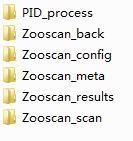
\includegraphics[width=3in]{ZooProcess_File_List}
    		\caption{目录列表}
    		\label{fig:FileList}
    		\end{figure}
		
		enter sample ID:例如001

		填充metadate:

		主要的内容如图~\ref{fig:FileContent1}和~\ref{fig:FileContent2}所示:
		\begin{figure}[!ht]
    		\centering
    		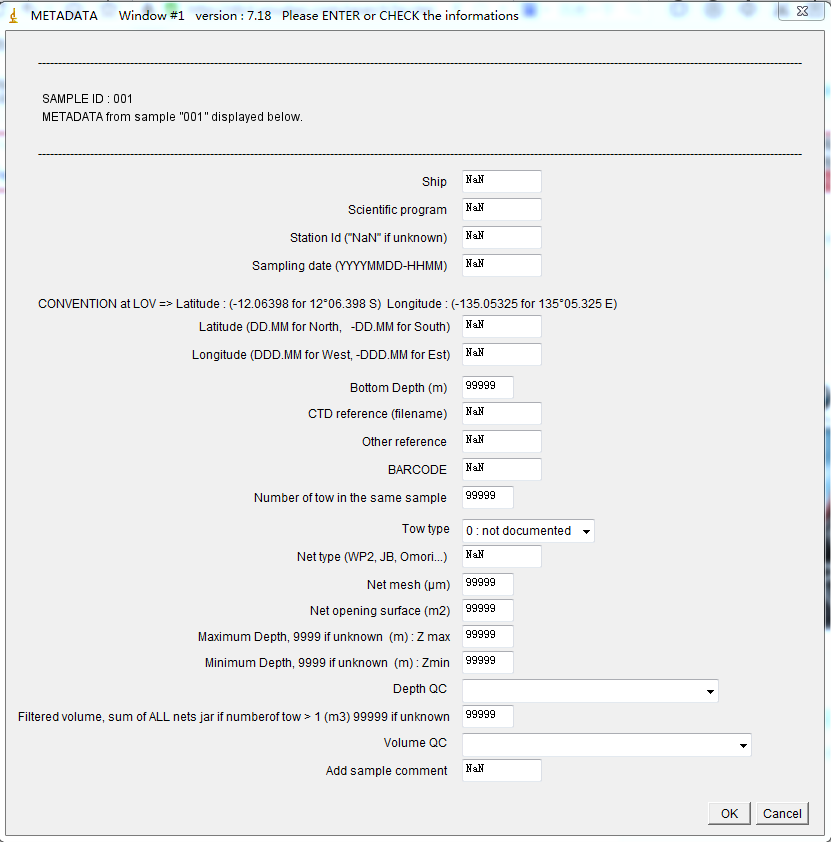
\includegraphics[width=7in]{ZooProcess_File_Content_1}
    		\caption{填充内容1}
    		\label{fig:FileContent1}
    		\end{figure}
		
		\begin{figure}[!ht]
    		\centering
    		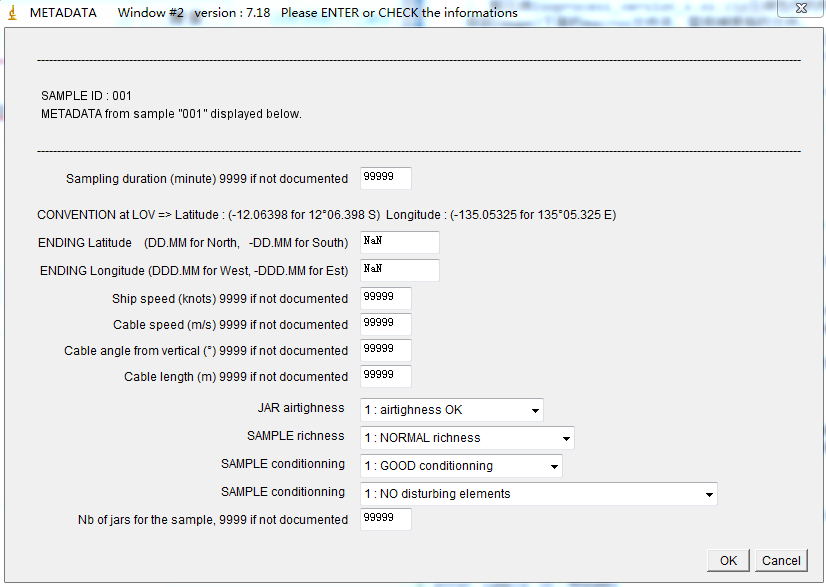
\includegraphics[width=7in]{ZooProcess_File_Content_2}
    		\caption{填充内容2}
    		\label{fig:FileContent2}
    		\end{figure}
		在这里需要我们填充很多信息,包括采样的地点、经度、纬度、采样网格的大小等参数,这些会在以后的log文件和meta元数据文件中写入。具体的条目我就不再详细介绍了,毕竟不是很明白。
	\subsubsection{使用一个例子项目来了解Zooprocess的工作流程。}
		\begin{enumerate}
			\item 下载例子,\href{http://www.obs-vlfr.fr/LOV/ZooPart/ZooScan/article.php3?id_article=219}{下载地址},下载“the project to be utilized with Zooprocess”这个条目对应的文件。
			\item 将下载下来的文件拷贝到Zooprocess的工作目录下,然后打开ImageJ,就可以选择我们下载下来的项目Zooscan\_rond\_carre\_zooprocess\_tp了。
			\item 选择好项目后,会进入到菜单选择窗口,用户在这里可以选择要进行的工作,在这里有两种工作模式User模式和Advanced模式,一般情况下我们选择User模式就好了,其他的选择默认。高级模式就是为用户提供了更多手动操作的步骤和功能,让用户可以更加全面的参与参数的修改等工作。
			
			两种模式包含的功能分别如图~\ref{fig:UserModel}和~\ref{fig:AdvancedModel}所示:~\\\\
				\begin{figure}[!ht]
    					\centering
    					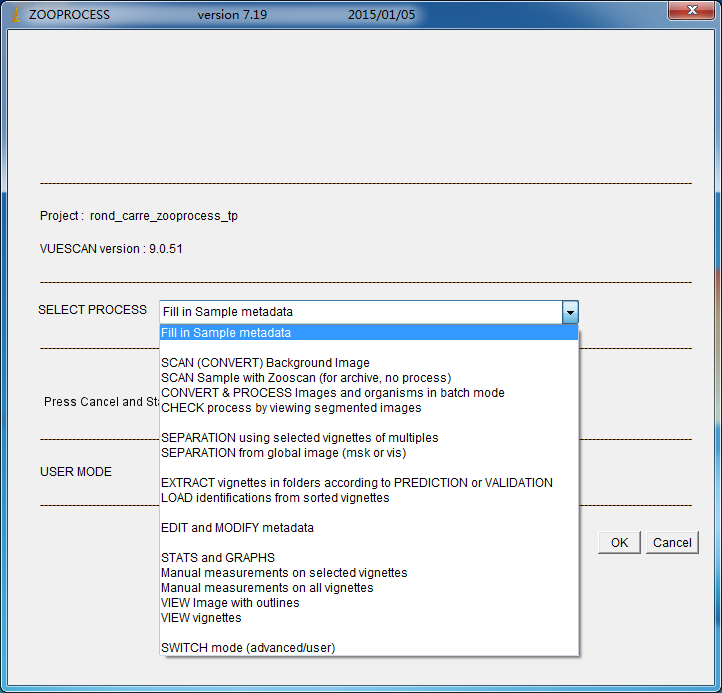
\includegraphics[width=6in]{ZooProcess_Model_User}
    					\caption{普通模式}
    					\label{fig:UserModel}
    				\end{figure}
				\begin{figure}[!ht]
    					\centering
    					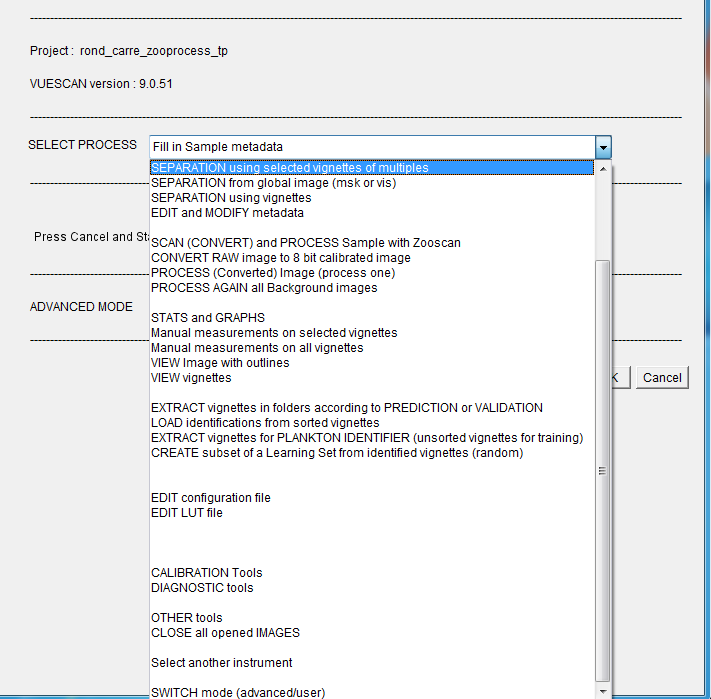
\includegraphics[width=6in]{ZooProcess_Model_Advanced}
    					\caption{高级模式}
    					\label{fig:AdvancedModel}
    				\end{figure}
			
			\item 进行处理的第一步就是需要扫描背景图像和扫描样本图像两项工作,在这里由于没有实际的ZooScan仪器,所以就跳过,直接进行下面的步骤,在下载的实例文件中已经为我们提供了示例的扫描后的样本图像和空白图像。分别保存在项目目录下面的Zooscan\_back和Zooscan\_scan目录下面。
				\begin{figure}[!ht]
    					\centering
    					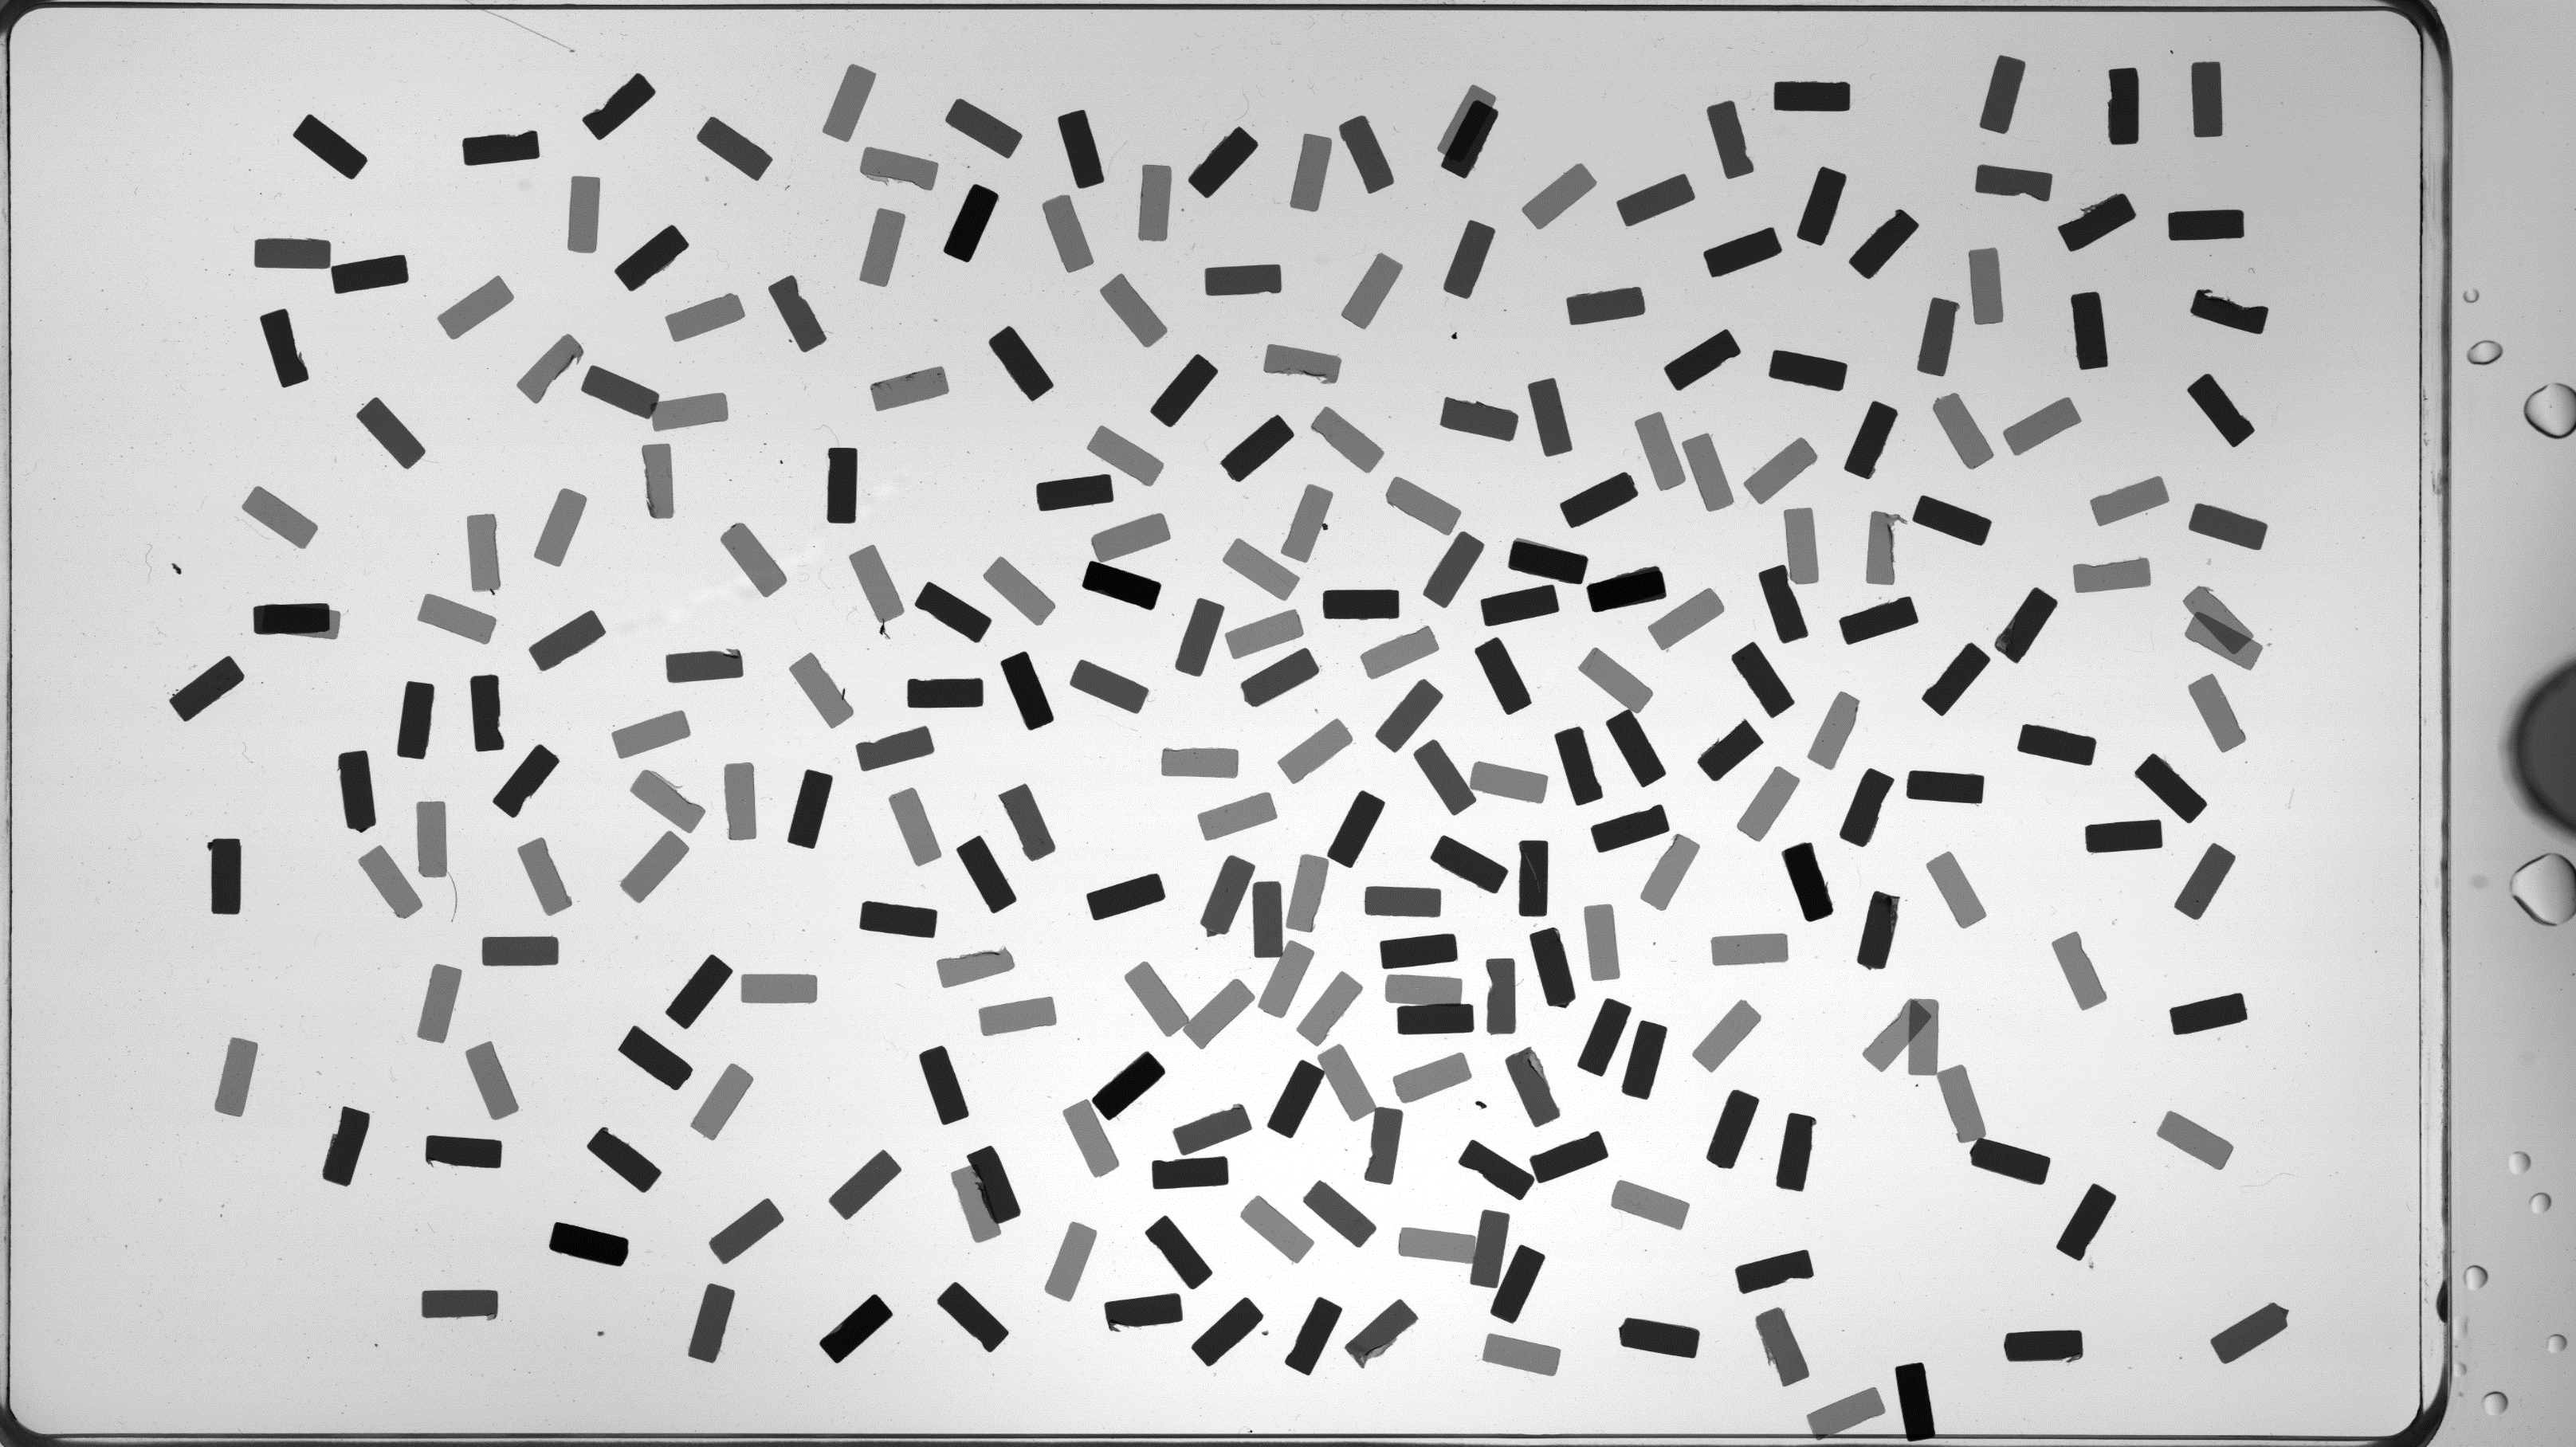
\includegraphics[width=4in]{ZooProcess_Sample}
    					\caption{样本图片}
    					\label{fig:Sample}
    				\end{figure}
				\begin{figure}[!ht]
    					\centering
    					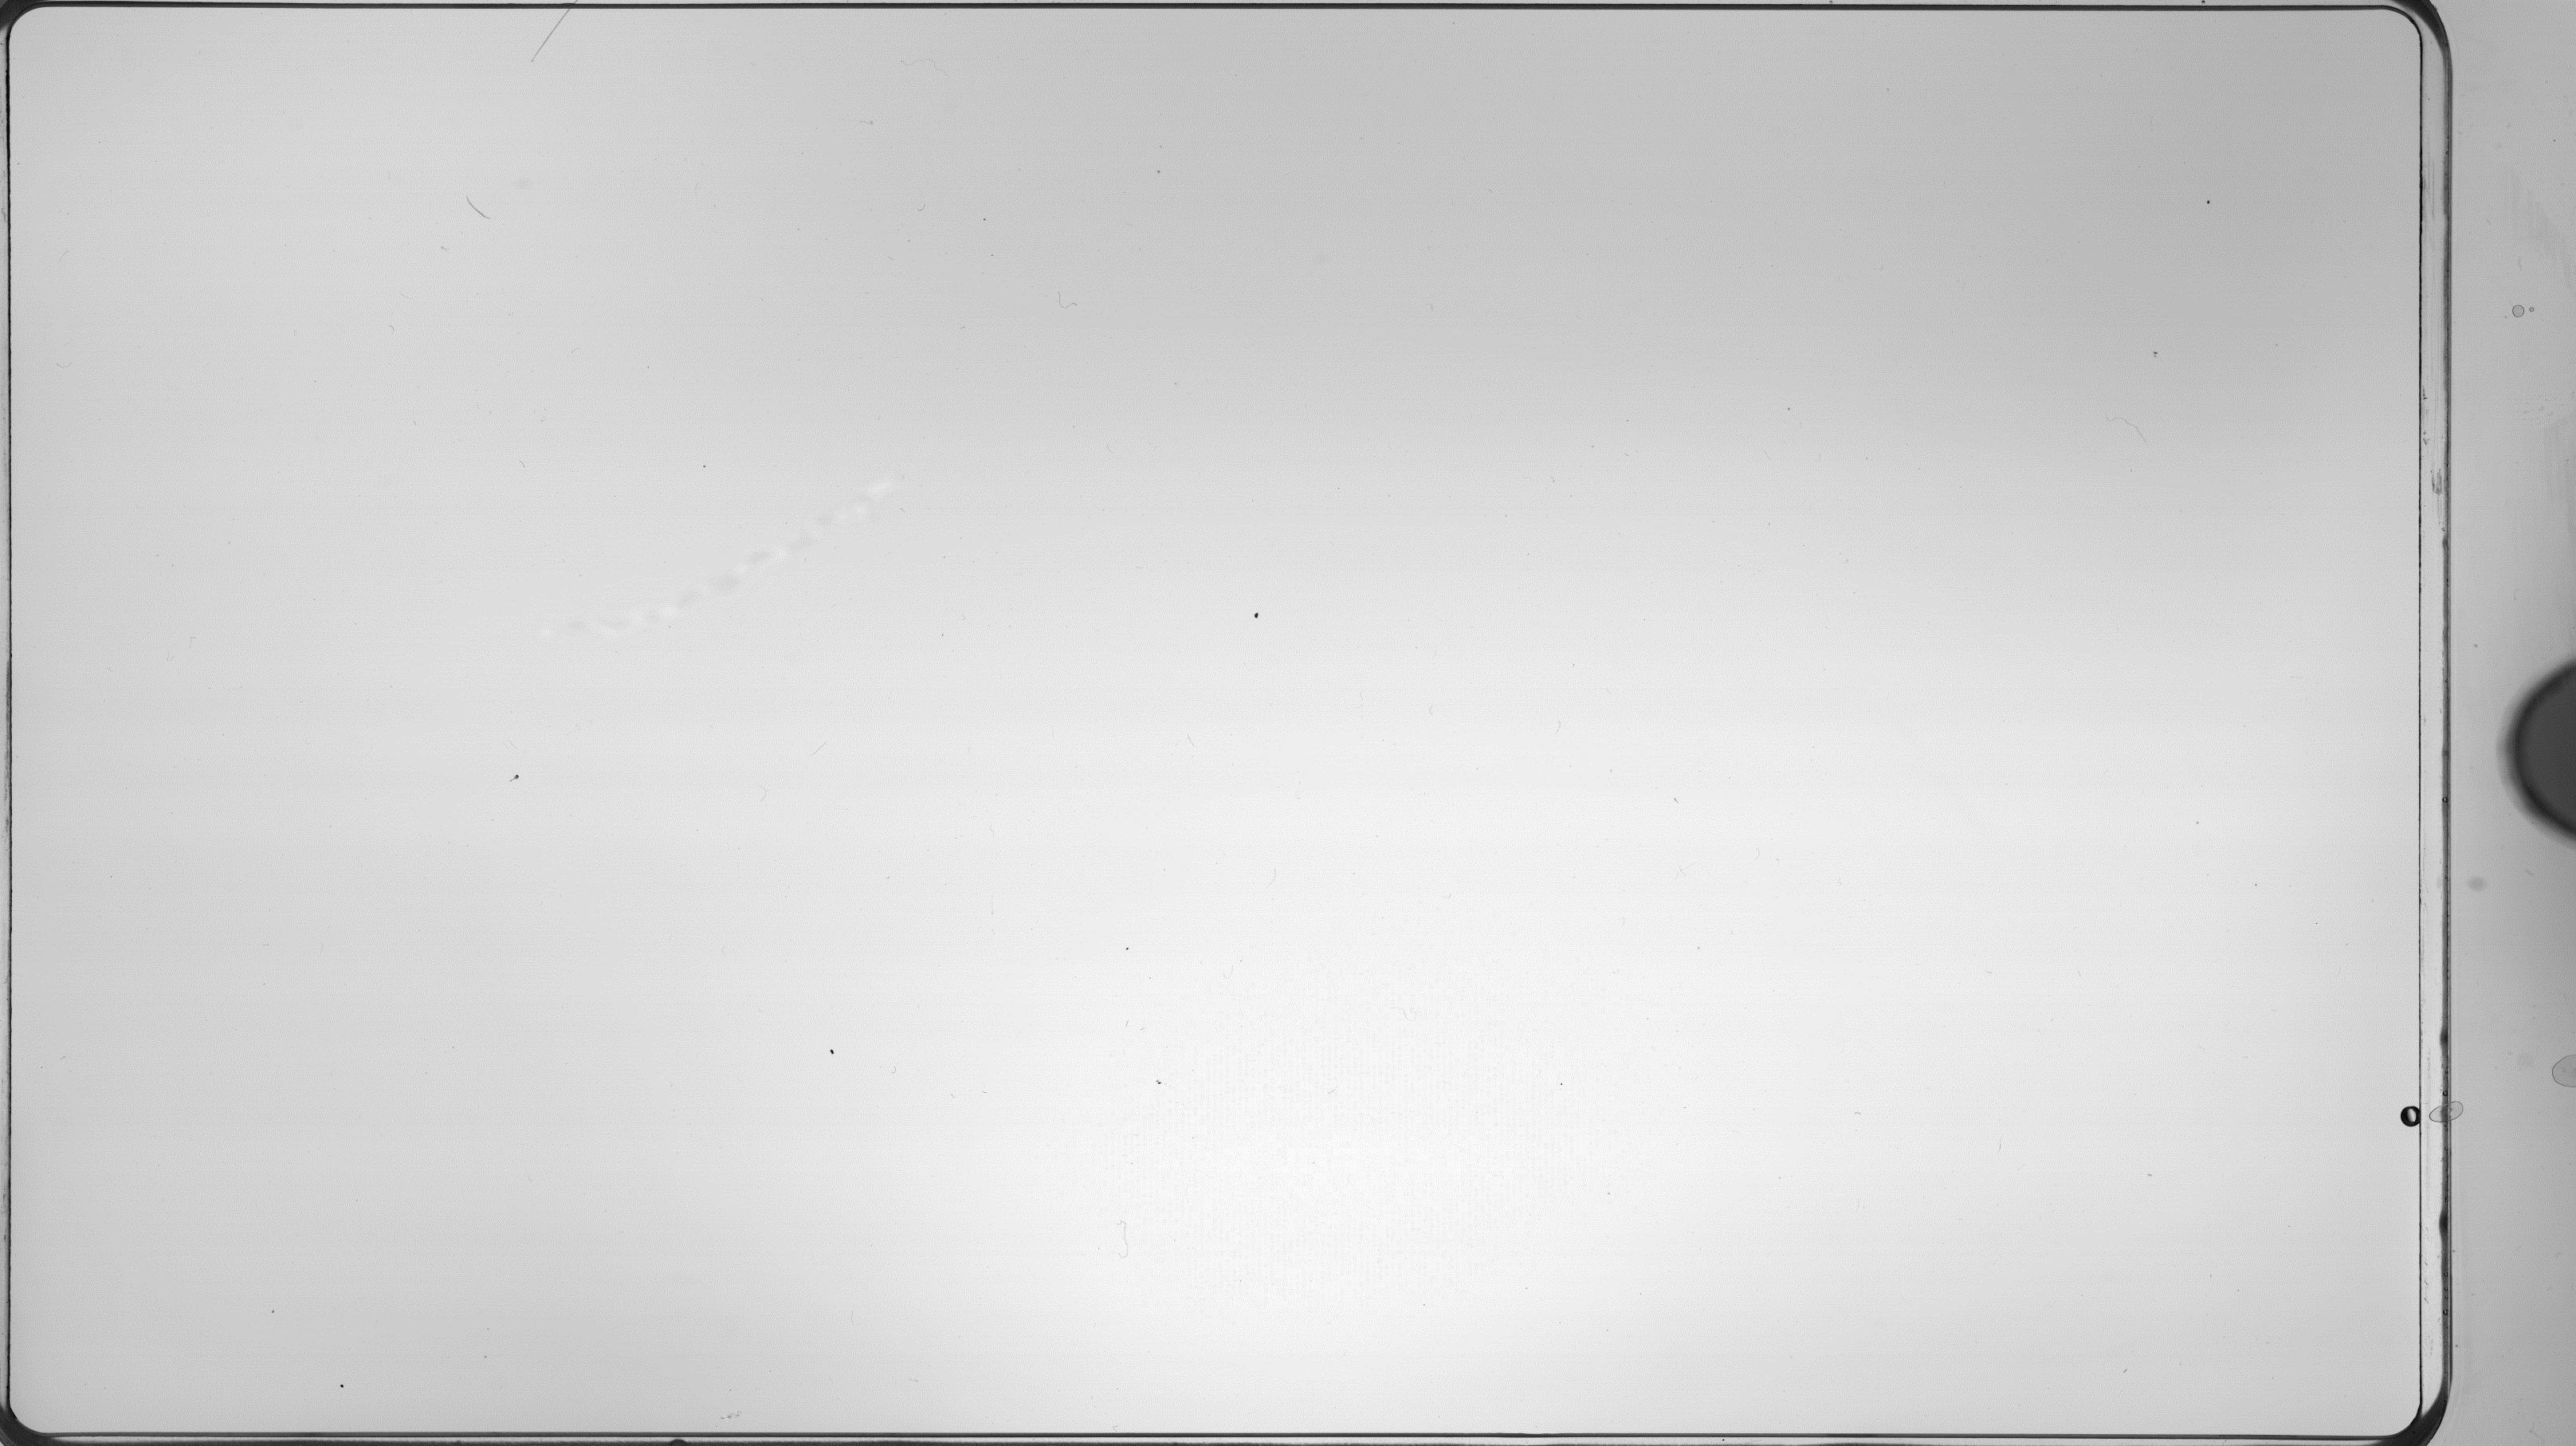
\includegraphics[width=4in]{ZooProcess_Sample_Background}
    					\caption{背景图片}
    					\label{fig:Background}
    				\end{figure}
				
				扫描后的样本的原始的.tif图像文件和log.txt记录文件和meta.txt元数据文件都会在path $\backslash$to $\backslash$project $\backslash$Zooscan\_scan $\backslash$\_raw目录下建立并存储。
				\begin{figure}[!ht]
    					\centering
    					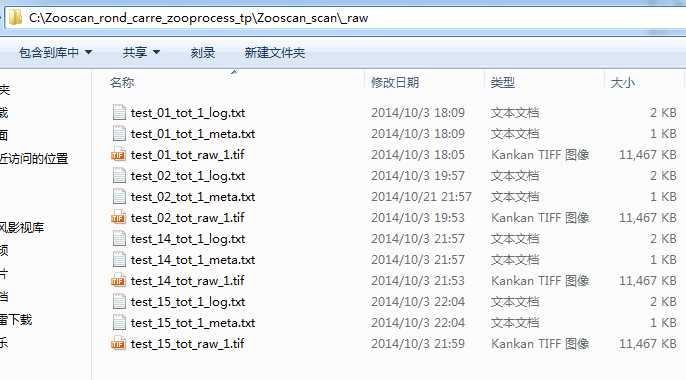
\includegraphics[width=5.5in]{ZooProcess_File_List_Raw}
    					\caption{文件列表}
    					\label{fig:FileListRaw}
    				\end{figure}
				\begin{itemize}
					\item log文件记录了扫描方法(参数)的信息。
					\item meta文件给出了采样方法(网格大小、质量)和ZooSCAN的准备(前置筛选和二次抽样率等)信息。
				\end{itemize}
			\item 在Zooprocess的主菜单中选择"Convert and process image in batch mode"选项来使用批处理的方法进行样本的处理和转换。
			
				这个过程会持续很长时间,做了很多的工作,从原图像中检测并且识别个体,并且把识别后的单个个体片段提取出来,以jpg的格式存储在$\backslash$path$\backslash$to$\backslash$project$\backslash$Zooscan\_scan$\backslash$\_work目录下。存储的文件除了每一个识别出来的个体片段外还包括原图像以及去掉背景后样本图和本次处理后对应的pid文件。这个.PID文件是后面数据分析的主要文件,它是一个连接了log.txt文件、meta.txt文件、应用的处理功能和meas.txt(一个包含所有目标(列)和测量值(行)的表格)文件的单一文件。测量值中可能会用于数据分析的计算值有Area,Major和Minor(同测量的目标拥有相同区域的椭圆的长轴和短轴)。其他测量值是用于自动识别目标的形状和结构的参数以及他们在托盘中的位置。除了work目录内,PID文件也被自动的复制到项目目录下的"PID\_Result"目录下。PID文件可以通过“PID Viewer”程序来查看。图~\ref{fig:Pid1}和~\ref{fig:Pid2}是PID文件的基本格式。
				\begin{figure}[!ht]
    					\centering
    					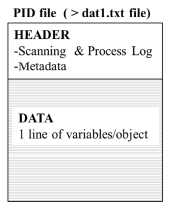
\includegraphics[width=2in]{ZooProcess_Pid1}
    					\caption{PID文件1}
    					\label{fig:Pid1}
    				\end{figure}
				\begin{figure}[!ht]
    					\centering
    					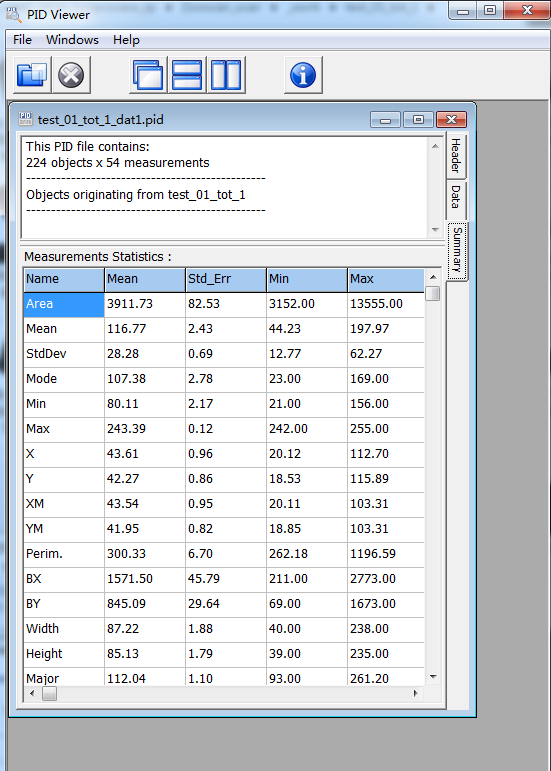
\includegraphics[width=5in]{ZooProcess_Pid2}
    					\caption{PID文件2}
    					\label{fig:Pid2}
    				\end{figure}
			\item 检查图像质量
				
				图像处理过后,必须检查背景是否是通过专用的工具从样本图像中被完全减去了。
	
				选择Zooprocess菜单中的“CHECK process by viewing segmented images”功能,手动检查每一张处理后的原图像。检查完后会给出一个checked的标识。

				如果对于图像质量依旧有疑问的话,可以继续通过“view image with outlines”和“view vignettes”两个工具来检查。这些工具可以让系统通过用户点击来来手动的判断是否是有多个生物体被检测成了一个单一的个体。
			\item 检查“接触问题”并且通过点击物体来分离图片上的物体。
				
				如果你对放在扫描托盘手动分离效果(很多个体在图像上接触在一起)不满意的话,还有如果你注意到很多的小片段上包含接触的目标或者很白图像上显示出很多接触的目标的话,你应该在图像上手动的添加分割。

	使用“SEPARATION from global image(msk or vis)”功能来分离接触在一起的生物体通过在他们之间用鼠标划线的方法。
			\item 分离后重新处理。
				
				完成了上面的分离之后,必须重新进行“CONVERT and PROCESS”步骤来使上面的分离方法生效并且得到新的结果。
		\end{enumerate}

